
\chapter{机器学习基础}

机器学习起源于上世纪50年代,1959年在IBM工作的Arthur Samuel设计了一个下棋程序,这个程序具有学习的能力,它可以在不断的对弈中提高自己。由此提出了“机器学习”这个概念,它是一个结合了多个学科如概率论,优化理论,统计等,最终在计算机上实现自我获取新知识,学习改善自己的这样一个研究领域。机器学习是人工智能的一个子集,目前已经发展出许多有用的方法,比如支持向量机,回归,决策树,随机森林,强化方法,集成学习,深度学习等等,一定程度上可以帮助人们完成一些数据预测,自动化,自动决策,最优化等初步替代脑力的任务。本章我们主要介绍下机器学习的基本概念、监督学习、分类算法、逻辑回归、代价函数、损失函数、LDA、PCA、决策树、支持向量机、EM算法、聚类和降维以及模型评估有哪些方法、指标等等。

\section{基本概念}

\subsection{大话理解机器学习本质}

机器学习(Machine Learning, ML),顾名思义,让机器去学习。这里,机器指的是计算机,是算法运行的物理载体,你也可以把各种算法本身当做一个有输入和输出的机器。那么到底让计算机去学习什么呢?对于一个任务及其表现的度量方法,设计一种算法,让算法能够提取中数据所蕴含的规律,这就叫机器学习。如果输入机器的数据是带有标签的,就称作有监督学习。如果数据是无标签的,就是无监督学习。

\subsection{什么是神经网络}

神经网络就是按照一定规则将多个神经元连接起来的网络。不同的神经网络,具有不同的连接规则。例如全连接(Full Connected, FC)神经网络,它的规则包括:

\begin{enumerate}
\item 有三种层:输入层,输出层,隐藏层。
\item 同一层的神经元之间没有连接。
\item fully connected的含义:第 N 层的每个神经元和第 N-1 层的所有神经元相连,第 N-1 层神经元的输出就是第 N 层神经元的输入。
\item 每个连接都有一个权值。
\end{enumerate}

{\bf 神经网络架构} 图\ref{fig:2.1}就是一个神经网络系统,它由很多层组成。输入层负责接收信息,比如一只猫的图片。输出层是计算机对这个输入信息的判断结果,它是不是猫。隐藏层就是对输入信息的传递和加工处理。

 %\begin{figure}[h]
 %  \centering
 %  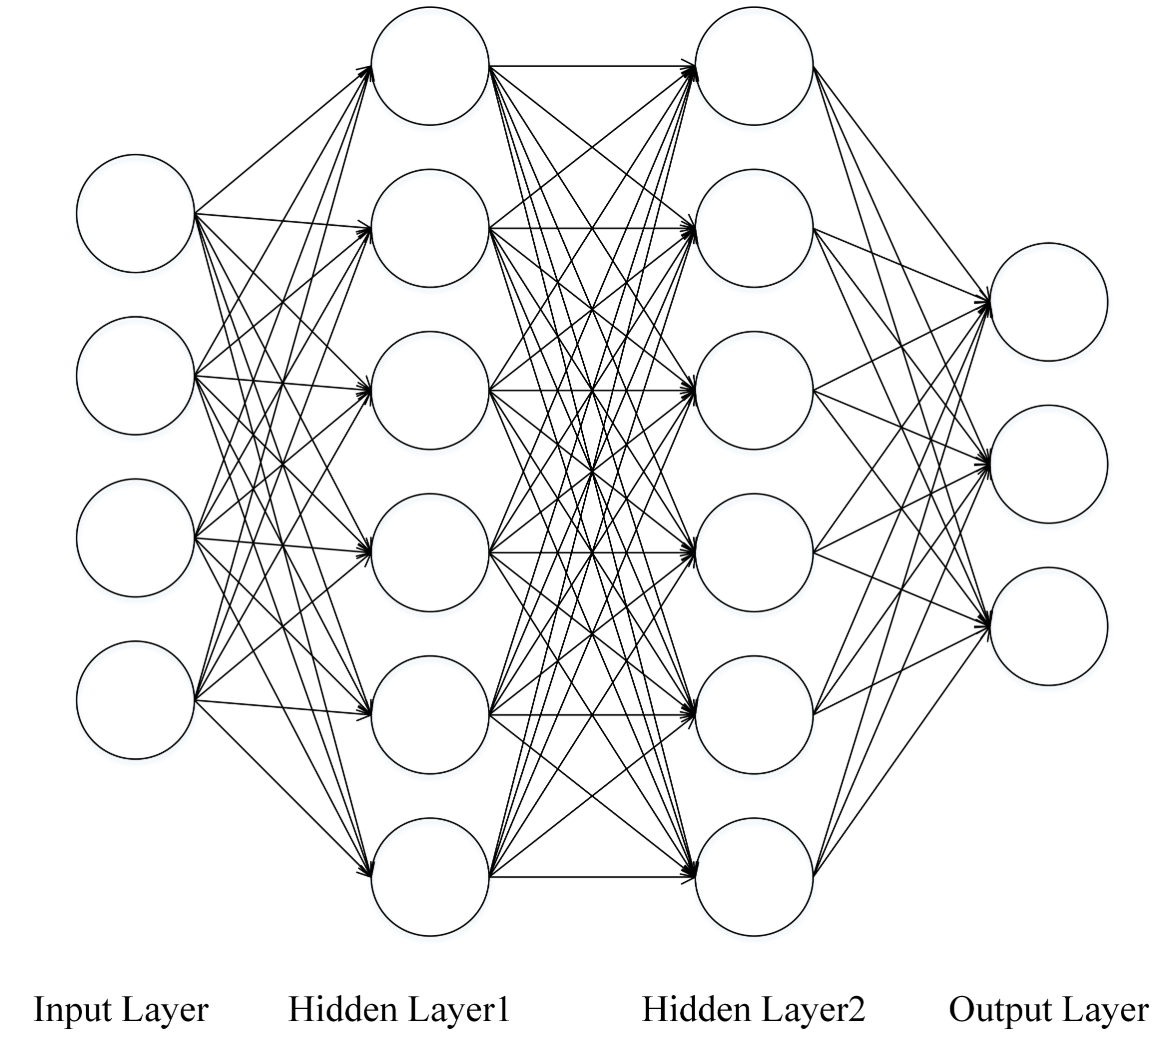
\includegraphics[width=.7\textwidth]{2.5.1.png}
 %  \caption{神经网络系统}
 %  \label{fig:2.1}
 %\end{figure}
